\chapter{User Interface Design}
\section{Mockups}
The only way to use the CKB platform is through the website. As previously mentioned in the RASD document the interfaces will be different according to the user who is using them, as the provided functionality are different. 

\subsection*{Used by all users.}
In figure \ref{fig:frontPage} is represented the initial page that all users visualize every time they open the website. The user can subsequently choose between "log in" in figure \ref{fig:login}, if he is already registered, or "sign up in figure \ref{fig:signup}.
\begin{figure}[h]
    \centering
    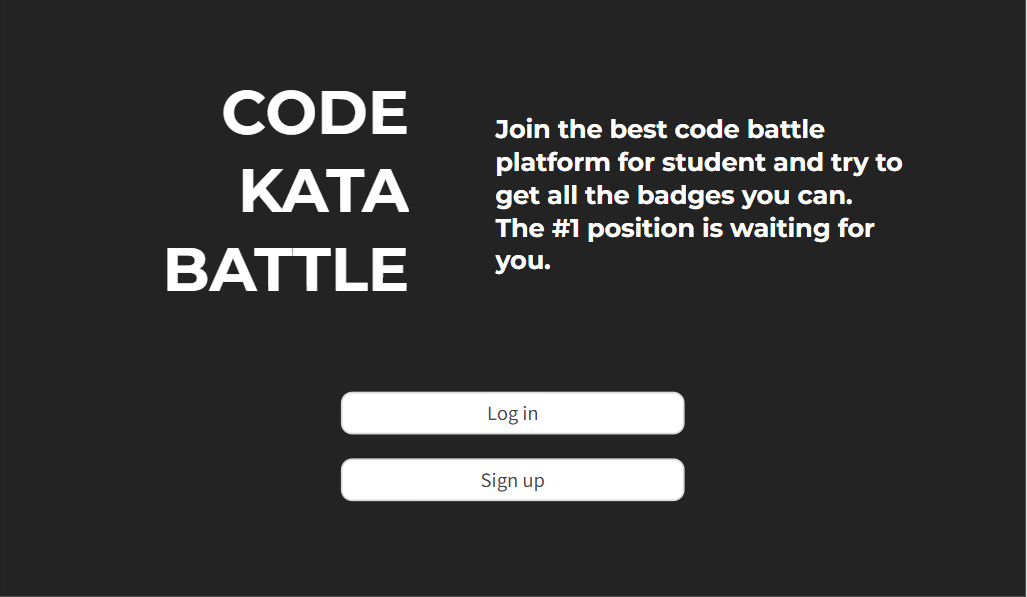
\includegraphics[width=\textwidth]{images/mockups/FrontPage.png}
    \caption{Front Page}
    \label{fig:frontPage}
\end{figure}
                                                                                
\begin{figure}[h]
    \centering
    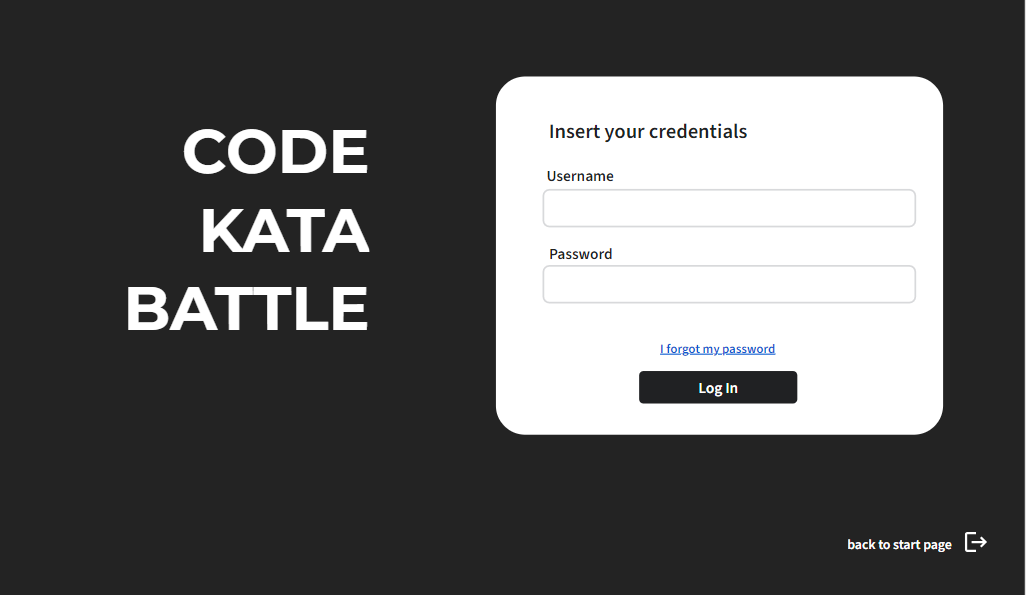
\includegraphics[width=\textwidth]{images/mockups/Login.png}
    \caption{Log in}
    \label{fig:login}
\end{figure}

\begin{figure}[h]
    \centering
    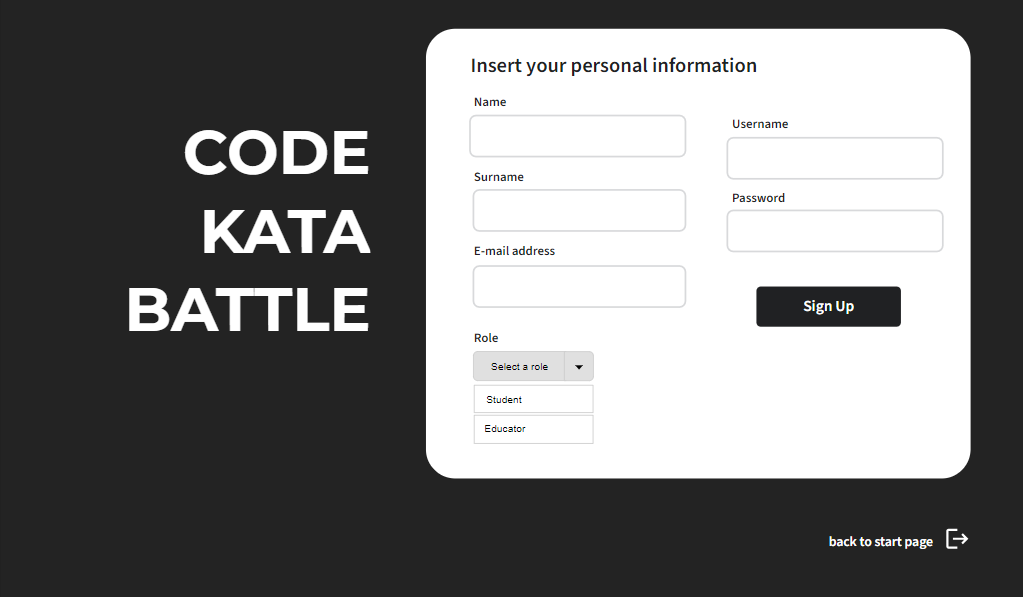
\includegraphics[width=\textwidth]{images/mockups/Signup.png}
    \caption{Sign up}
    \label{fig:signup}
\end{figure}
\clearpage

Another feature available to both students and educators is the ability to view all tournaments and their rankings. By selecting a tournament in the all tournaments page in figure \ref{fig:allT}, the user is able to see its ranking and all active badges as in figure \ref{fig:dashT}.
\begin{figure}[h]
    \centering
    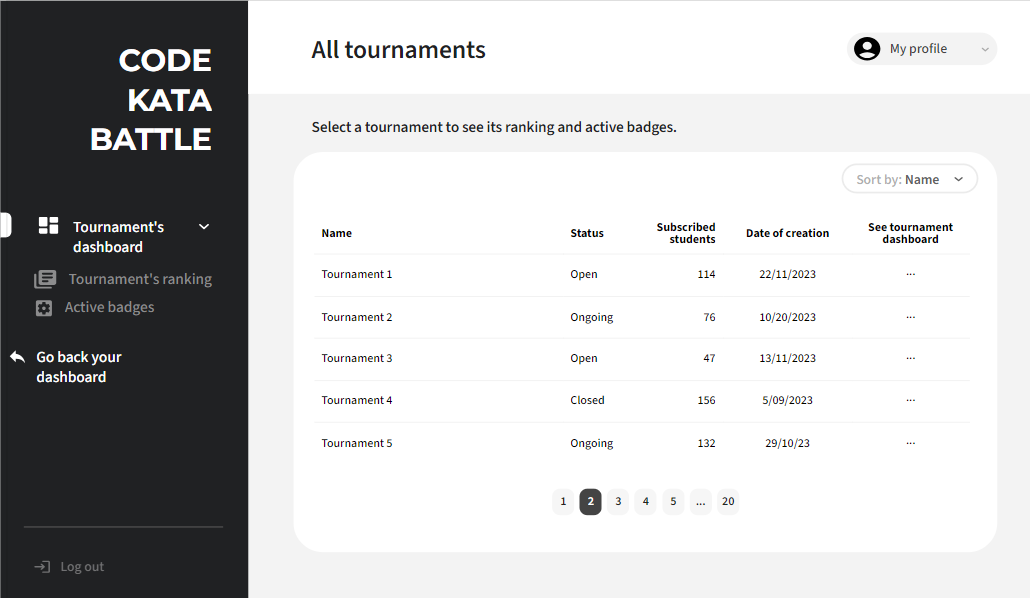
\includegraphics[width=\textwidth]{images/mockups/AllTournaments.png}
    \caption{All tournaments}
    \label{fig:allT}
\end{figure}

\begin{figure}[h]
    \centering
    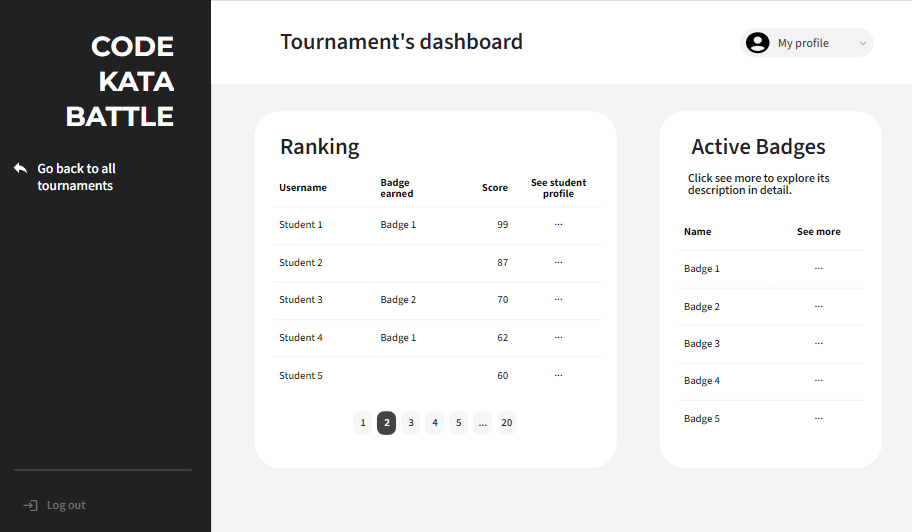
\includegraphics[width=\textwidth]{images/mockups/TournamentDashboard.png}
    \caption{Tournament dashboard}
    \label{fig:dashT}
\end{figure}

To view a student's profile, the users will have a function in the general dashboard. They must type the username in the field and then search for it.
\clearpage

\subsection*{Used by the educators.}
From the general dashboard the educator will be able to use the CKB platform in all its functionality. 
\begin{figure}[h]
    \centering
    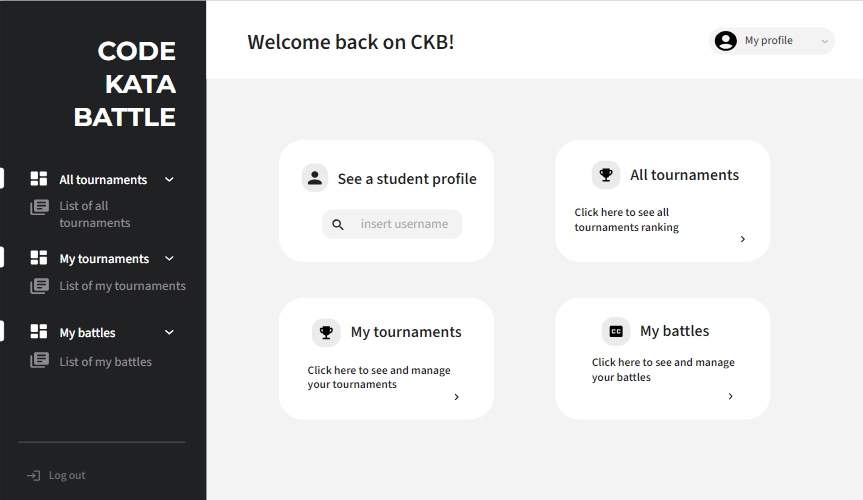
\includegraphics[width=\textwidth]{images/mockups/educators/Edashboard.png}
    \caption{Educator's dashboard}
    \label{fig:dashE}
\end{figure}

By compiling all the fields in the "Create a tournament" page in figure \ref{fig:createT} the educator is able to create a tournament and badges.
\begin{figure}[h]
    \centering
    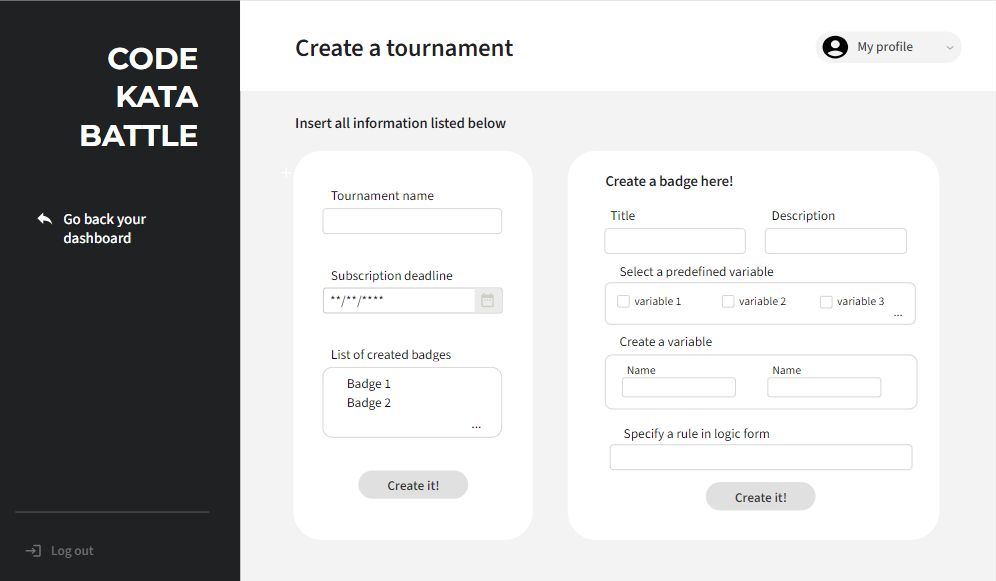
\includegraphics[width=\textwidth]{images/mockups/educators/createT.png}
    \caption{Create tournament}
    \label{fig:createT}
\end{figure}
\clearpage

From the "My tournaments" page in figure \ref{fig:EmyT} the educator is able to manage them. By clicking on one tournament the educator will enter the page "manage tournament" in figure \ref{fig:manageT}.
\begin{figure}[h]
    \centering
    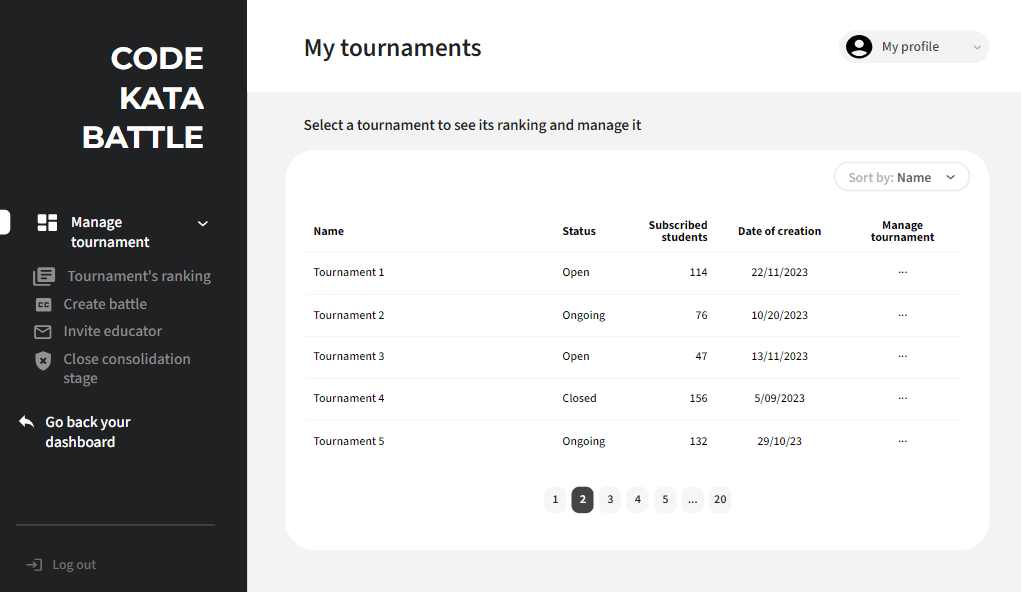
\includegraphics[width=\textwidth]{images/mockups/educators/MyTournaments.png}
    \caption{Educator's tournaments}
    \label{fig:EmyT}
\end{figure}

\begin{figure}[h]
    \centering
    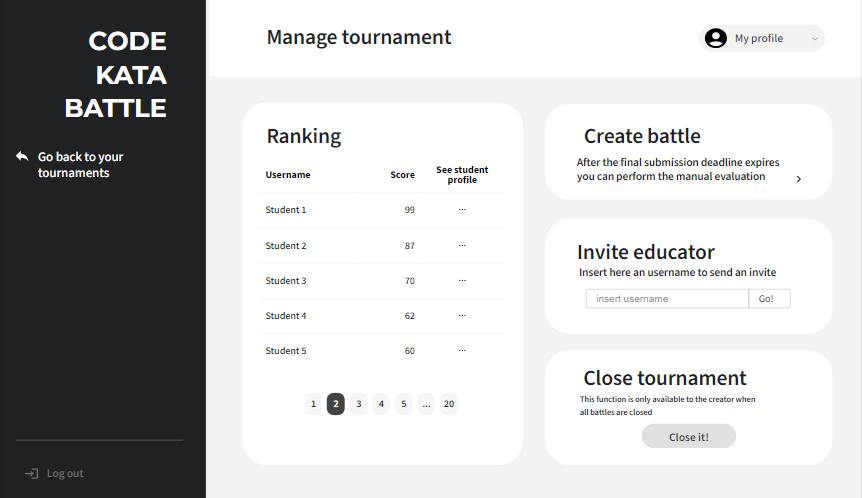
\includegraphics[width=\textwidth]{images/mockups/educators/ManageTournament.png}
    \caption{Manage tournament}
    \label{fig:manageT}
\end{figure}
\clearpage

By compile all the fields in the "Create a battle" page in figure \ref{fig:createB} the educator is able to create a battle in the tournament he/she has selected before.
\begin{figure}[h]
    \centering
    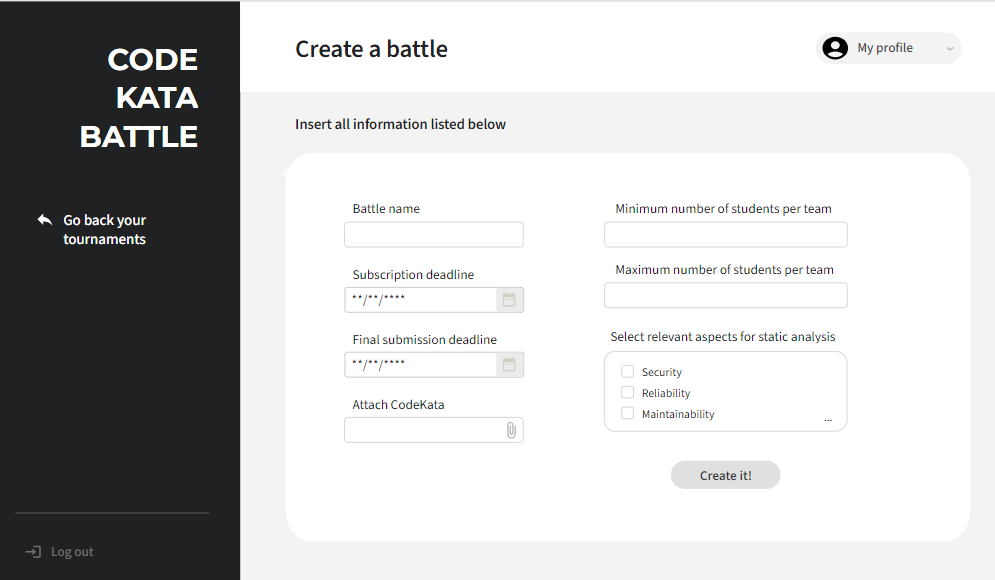
\includegraphics[width=\textwidth]{images/mockups/educators/createB.png}
    \caption{Create battle}
    \label{fig:createB}
\end{figure}

From the "My battle" page in figure \ref{fig:EmyB} the educator is able to manage them. By clicking on one battle the educator will enter the page "manage battle" in figure \ref{fig:manageB}.
\begin{figure}[h]
    \centering
    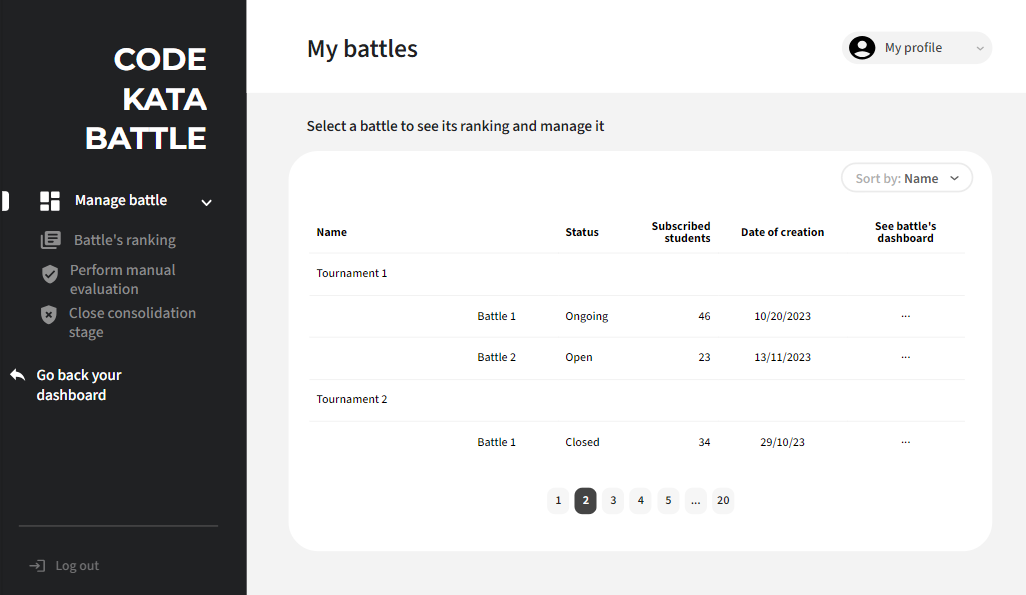
\includegraphics[width=\textwidth]{images/mockups/educators/MyBattles.png}
    \caption{Educator's battle}
    \label{fig:EmyB}
\end{figure}

\begin{figure}[h]
    \centering
    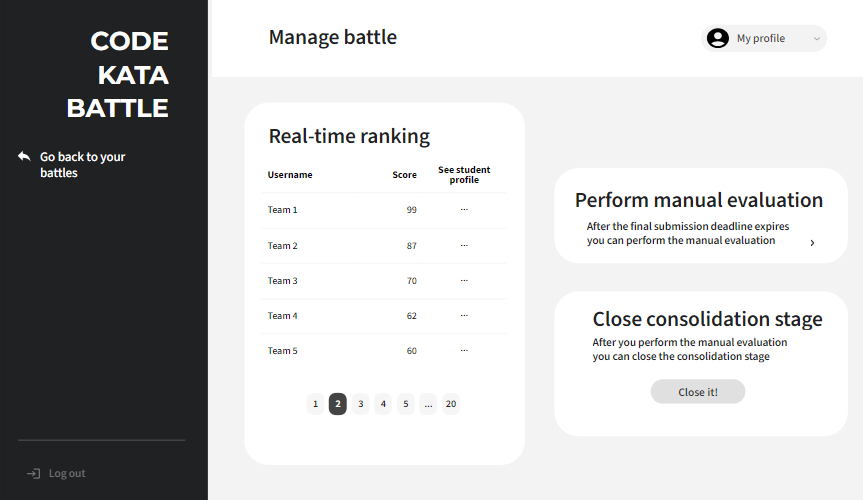
\includegraphics[width=\textwidth]{images/mockups/educators/ManageBattle.png}
    \caption{Manage battle}
    \label{fig:manageB}
\end{figure}

The educator can perform the manual evaluation only for his/hers battles. As in figure \ref{fig:evalM} the educator is requested to insert an evaluation for each student enrolled in the battle.
\begin{figure}[h]
    \centering
    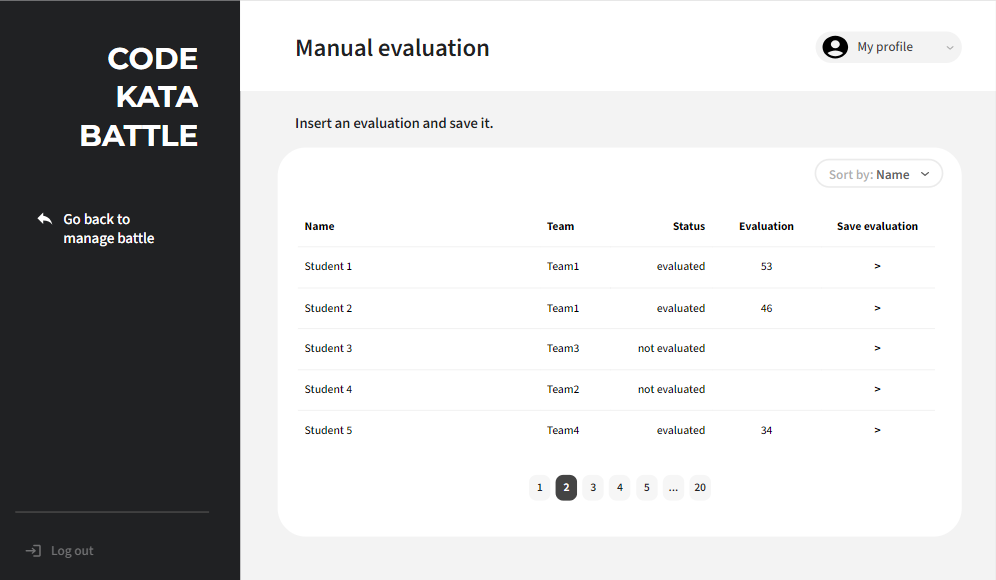
\includegraphics[width=\textwidth]{images/mockups/educators/evalM.png}
    \caption{Manual evaluation}
    \label{fig:evalM}
\end{figure}

\clearpage
\subsection*{Used by the students.}
From the general dashboard the student will be able to use the CKB platform in all its functionality. 
\begin{figure}[h]
    \centering
    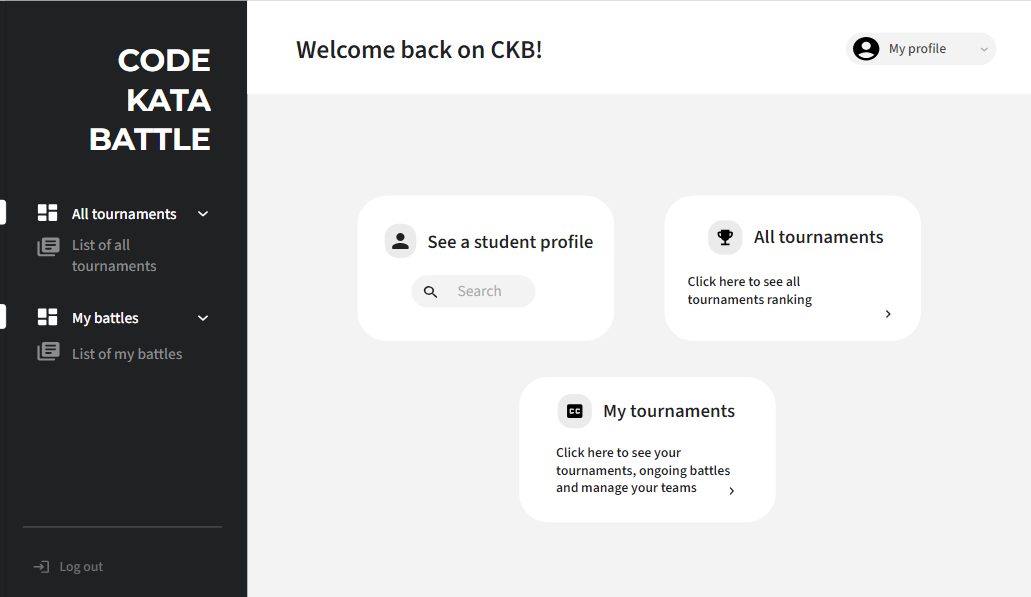
\includegraphics[width=\textwidth]{images/mockups/students/Sdashboard.png}
    \caption{Student's dashboard}
    \label{fig:Sdash}
\end{figure}

From the "My tournaments" page in figure \ref{fig:SmyT} the student is able to manage his/hers battles by clicking on one of them. The student will enter the page "manage battle" in figure \ref{fig:battleDash} from which he/she can manage his tournaments
\begin{figure}[h]
    \centering
    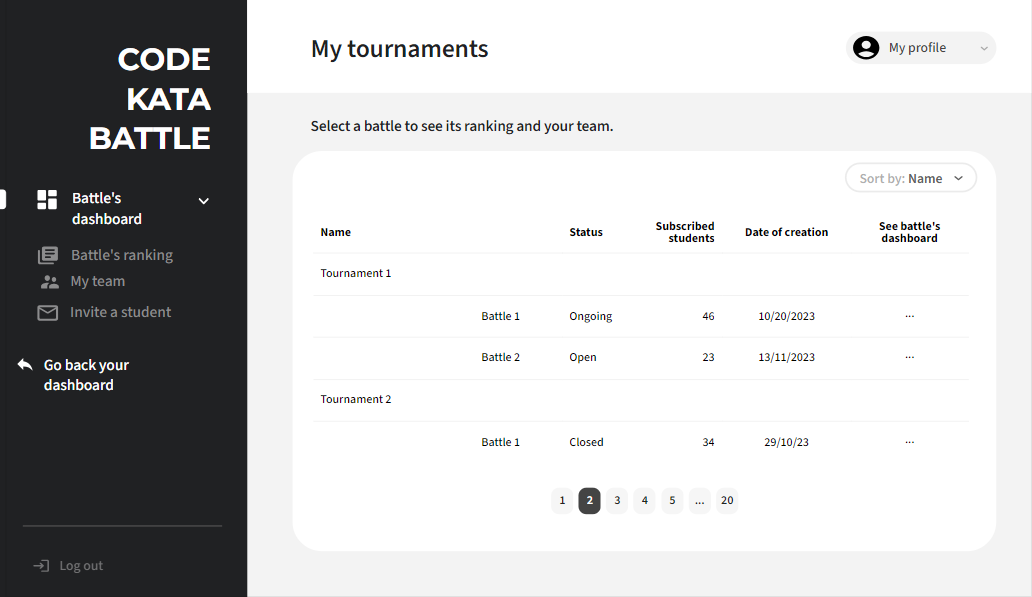
\includegraphics[width=\textwidth]{images/mockups/students/MyTournaments.png}
    \caption{Student's tournaments}
    \label{fig:SmyT}
\end{figure}

\begin{figure}[h]
    \centering
    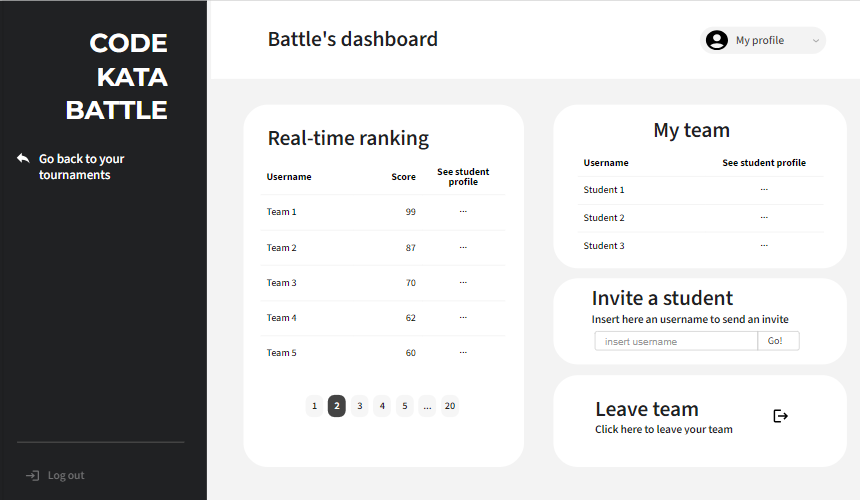
\includegraphics[width=\textwidth]{images/mockups/students/BattleDashboard.png}
    \caption{Battle dashboard}
    \label{fig:battleDash}
\end{figure}

